\documentclass[11pt,fleqn]{article}
\usepackage[margin=1in,top=1in,bottom=1in]{geometry}
\usepackage{tikz}
\usepackage{mathtools}
\usepackage{longtable}
\usepackage{enumitem}
\usepackage{hyperref}
%\usepackage[dvips]{graphics}
%\usepackage[table]{xcolor}
%\usepackage{amssymb}
\usepackage{float}
%\usepackage{subfig}
\usepackage{booktabs}
\usepackage{subcaption}

\usepackage[normalem]{ulem}

\usepackage{multicol}
\usepackage{txfonts}
\usepackage{amsfonts}
\usepackage{natbib}
\usepackage{gb4e}
\usepackage[all]{xy}
\usepackage{rotating}
\usepackage{tipa}
\usepackage{multirow}
\usepackage{authblk}
\usepackage{url}
\usepackage{pdflscape}
\usepackage{rotating}
\usepackage{adjustbox}
\usepackage{array}

\def\bad{{\leavevmode\llap{*}}}
\def\marginal{{\leavevmode\llap{?}}}
\def\verymarginal{{\leavevmode\llap{??}}}
\def\swmarginal{{\leavevmode\llap{4}}}
\def\infelic{{\leavevmode\llap{\#}}}

\definecolor{airforceblue}{rgb}{0.36, 0.54, 0.66}
%\definecolor{gray}{rgb}{0.36, 0.54, 0.66}

\newcommand{\dashrule}[1][black]{%
  \color{#1}\rule[\dimexpr.5ex-.2pt]{4pt}{.4pt}\xleaders\hbox{\rule{4pt}{0pt}\rule[\dimexpr.5ex-.2pt]{4pt}{.4pt}}\hfill\kern0pt%
}

\setlength{\parindent}{.3in}
\setlength{\parskip}{0ex}

\newcommand{\yi}{\'{\symbol{16}}}
\newcommand{\nasi}{\~{\symbol{16}}}
\newcommand{\hina}{h\nasi na}
\newcommand{\ina}{\nasi na}

\newcommand{\foc}{$_{\mbox{\small F}}$}

\hyphenation{par-ti-ci-pa-tion}

\setlength{\bibhang}{0.5in}
\setlength{\bibsep}{0mm}
\bibpunct[:]{(}{)}{,}{a}{}{,}

\newcommand{\6}{\mbox{$[\hspace*{-.6mm}[$}} 
\newcommand{\9}{\mbox{$]\hspace*{-.6mm}]$}}
\newcommand{\sem}[2]{\6#1\9$^{#2}$}
\renewcommand{\ni}{\~{\i}}

\newcommand{\citepos}[1]{\citeauthor{#1}'s \citeyear{#1}}
\newcommand{\citeposs}[1]{\citeauthor{#1}'s}
\newcommand{\citetpos}[1]{\citeauthor{#1}'s (\citeyear{#1})}

\newcolumntype{R}[2]{%
    >{\adjustbox{angle=#1,lap=\width-(#2)}\bgroup}%
    l%
    <{\egroup}%
}
\newcommand*\rot{\multicolumn{1}{R{90}{0em}}}% no optional argument here, please!


\title{Higher-probability content is more projective than lower-probability content}

%\thanks{For helpful comments on the research presented here, we thank the audience at the 2018 Annual Meeting of XPRAG.de and at the University of T\"ubingen. We gratefully acknowledge financial support for this research from {\em National Science Foundation} grant BCS-1452674 (JT) and the Targeted Investment for Excellence Initiative at The Ohio State University (JT). IGOR Tuebingen}}

\author{Author(s)}

%\author[$\bullet$]{Judith Degen}
%\author[$\circ$]{Judith Tonhauser}

%\affil[$\bullet$]{Stanford University}
%\affil[$\circ$]{The Ohio State University / University of Stuttgart}

\renewcommand\Authands{ and }

\newcommand{\jt}[1]{\textbf{\color{blue}JT: #1}}

\begin{document}

%\tableofcontents
%\newpage

\maketitle

\vspace*{-1cm}

\begin{abstract}

abstract

\end{abstract}

			
\section{Introduction}\label{s1}

people?s individual beliefs are indicative of their prior probability

H: people?s prior beliefs about content affect project
Way 1: we measured the belief on one group of people, test how the average belief of that group, predict something about projection of the second ground
Way 2: assess within each participant?

\jt{We need an introduction that talks about how speakers and listeners are sensitive to prior probabilities assigned to events in using and interpreting language.} Events differ in how likely they are: for instance, if Sam is a broke college student, then the event of Sam buying a coffee is more likely than Sam buying a BMW. Subjective prior probabilities assigned to events, has been shown to affect interpretation in ways captured by models of language use that treat interpretation as Bayesian reasoning about an observed utterance (see, e.g., Franke \& J\"ager, 2016; Goodman \& Frank, 2016).



\begin{exe}
\ex 
\begin{xlist}
\ex Jane knows that Sam has a new hat.
\ex Jane thinks that Sam has a new hat.
\end{xlist}
\end{exe}

In making utterances, speakers present themselves as committed to the truth of some utterance content and as not committed to the truth of other utterance content.

\begin{exe}
\ex
\begin{xlist}
\ex Mary's daughter stopped biting her nails.
\ex Has Mary's daughter stopped biting her nails?
\end{xlist}
\end{exe}

projective content: content that a speaker presents themselves as committed to

stop nails 0.79

Has Mary?s daughter stopped biting her nails?

Mary's daughter has been biting her nails

stop play 0.89

Did Jack stop playing outside with the kids?

Jack was playing outside with the kids


\newpage

- does the prior probability of content influence its projectivity?

We investigate this question based on content at the center of research on projection:

- factive predicates: projective CC, but there's variability

- optionally factive predicates: projective, but less so than with factive predicaes

- non-factive: CC taken to be non-projective, but suggestive evidence to the contrary and perhaps with higher probability content, we can get some speaker commitment?

\newpage

In making utterances, speakers present themselves as committed to the truth of some utterance content and as not committed to the truth of other utterance content. For example, if a speaker utters the polar question in (\ref{proj}), they may be committed to the truth of the content of the complement, that Sam has a new hat, but they are likely not committed to the main clause content, that Jane knows of Sam's new hat; rather, this is the content they are asking about.

\begin{exe}
\ex\label{proj} Does Jane know that Sam has a new hat?
\end{exe}
One cue that listeners rely on in identifying which content speakers present themselves as committed to are the expressions uttered. If, for example, a speaker utters the variant of (\ref{proj}) with {\em think}, given in (\ref{proj2}), then the speaker is typically committed neither to the content of the complement nor to the main clause content. 

\begin{exe}
\ex\label{proj2} Does Jane think that Sam has a new hat?
\end{exe}
The inference to the truth of the content of the complement has long been taken to categorize clause-embedding predicates: the inference is typically taken to arise with factive predicates, like {\em know}, but not with non-factive predicates, like {\em think} (\citealt{kiparsky-kiparsky70,karttunen71b}, i.a.). However, \citealt*{tbd-variability} recently showed that there is variability among factive predicates in the inference to the truth of the content of the complement. One source of variability was the factive predicate: for instance, the inference was less likely to arise with {\em reveal} than with {\em discover}; for both of these predicates it was less likely than with {\em know}. Another source of variability was the lexical content of the clausal complement, that is, whether content of the complement was `Sam has a new hat', as in (\ref{proj}), or `Sam has a new BMW'. The authors hypothesized that the inference to the truth of the content of the complement may depend on its prior subjective probability, such that the inference to the truth of the content of the complement is more likely to arise the higher its prior probability. This paper provides support for this hypothesis in an experimental investigation of the contents of the complements of 20 English clause-embedding predicates for which the prior probability was systematically manipulated. 

\footnote{\label{f-github}The experiments, data and R code for generating the figures and analyses of the experiments reported on in this paper are available at [redacted for review].}
%\url{https://github.com/judith-tonhauser/factivity}.}  

\citealt{stevens-etal2017}: ``We also observed that the influence of prosody on the projectivity of the prejacent was heterogeneous across items. This observation suggests enriching the model with information about listeners? prior expectations about the prejacent, e.g., about how likely some- body is to smile given that they didn?t smile cheerfully.'' (p.1149)

\newpage

\paragraph{Previous work} The influence of prior probability on projection was previously investigated in \citealt{lorson2018} and \citealt{mahler2020}. \citet{lorson2018} investigated the influence of prior probability on the projectivity of the pre-state content of the English change of state verb {\em stop}: in the polar questions in (\ref{lorson-stim}), the pre-state contents are that James has worked as a plumber, in (\ref{lorson-stim}a), and that Linda has worked as a plumber, in (\ref{lorson-stim}b).

\begin{exe}
\ex\label{lorson-stim} 
\begin{xlist}
\ex Did James stop working as a plumber?
\ex Did Linda stop working as a plumber? \hfill (\citealt[38]{lorson2018})
\end{xlist}
\end{exe}
On each trial of \citepos{lorson2018} experiment, a speaker uttered a sentence like those in (\ref{lorson-stim}) to a listener. Gender stereotypes reported in \citealt{boyce-etal2018} were used to manipulate the prior probability of the pre-state content, that is, the prior beliefs of the interlocutors about the pre-state content: it is, for instance, more likely for a man (like James) to be a plumber than for a woman (like Linda) to be a plumber. The hypothesis was that higher probability pre-state contents, as in (\ref{lorson-stim}a), were more projective than lower probability pre-state contents, as in (\ref{lorson-stim}b). \citet{lorson2018} did not find empirical support for this hypothesis.

\citet{mahler2020} investigated the influence of prior probability on the projectivity of the content of the complement of clause-embedding predicates. The examples in (\ref{mahler-stim}) feature the clause-embedding predicate {\em know} which is embedded under negation, together with its clausal complements: the content of the clausal complement in (\ref{mahler-stim}a) is that Obama improved the American economy and in (\ref{mahler-stim}b) that Obama damaged the American economy.

\begin{exe}
\ex\label{mahler-stim} Cindy doesn't know that\ldots
\begin{xlist}
\ex \ldots Obama improved the American economy.
\ex \ldots Obama damaged the American economy. \hfill (\citealt[779]{mahler2020})
\end{xlist}
\end{exe}
On each trial of \citepos{mahler2020} experiment, the speaker who uttered a sentence like those in (\ref{mahler-stim}) was attending a meeting of the Democrat or the Republican party. The combination of the political party affiliation of the interlocutors and the content of the complement was used to manipulate the prior probability of the content: when the content of the complement was consistent with a liberal political perspective, as in (\ref{mahler-stim}a), it had a higher prior probability with Democrat interlocutors than with Republican interlocutors, and when the content of the complement was consistent with a conservative political perspective, as in (\ref{mahler-stim}b), it had a higher prior probability with Republican interlocutors than with Democrat interlocutors. \citet{mahler2020} found that prior probability influenced projection: the content of the complement was more projective when it had a higher prior probability than when it had a lower prior probability. 

\begin{itemize}

\item Both \citealt{lorson2018} and \citealt{mahler2020} used the `certain that' diagnostic for projection (\citealt{tbd-variability}).

\item Neither Lorson nor Mahler collected prior probability ratings from the participants: Lorson relied on \citealt{boyce-etal2018} and Mahler did a norming study.

\item Prior probability entered Lorson's model in a non-categorical fashion in Lorson 2018 (consistency measure) and in a categorical fashion in Mahler 2020 (political party (2 levels) and political orientation of CC (liberal vs.\ conservative). 

Lorson, p.36: ``The consistency measure is a value that ranges from 0 to 1, where a value close to 0 means that the gender of an individual is inconsistent with a certain occupation, according to the collected gender-bias that was found to be associated with that occupation. A value close to 1 means that the gender of an individual is consistent with an occupation.''

\end{itemize}

Mahler also manipulated clause-embedding predicate: two categories (factive: {\em know, realize, see, discover} and non-factive: {\em believe, think, feel}). CCs of factive predicates more projective than CCs of non-factive predicates. In addition to wanting to identify whether prior probability influences projection, she also wants to find out whether this only happens for factive predicates or for factive and non-factive predicates alike. Later on in the paper she adds the RQ of whether projection is influenced by factivity. She finds that prior probability influences projection for both factive and non-factives.  She also finds that projection is higher with factive than non-factive predicates. She concludes: ``CCs were more projective when the predicate was factive compared to when it was non-factive, regardless of the speaker?s political affiliation. This finding is compatible with the assumption that factive predicates lexically-encode their complements as presuppositions, whereas non-factive predicates do not.'' (p.788)

\newpage

\paragraph{Predicates we used}

The 20 predicates we investigated are listed in (\ref{pred}) with the categories they are typically taken to fall into: factive predicates in (\ref{pred}a), non-factive predicates in (\ref{pred}b) and optionally factive predicates in (\ref{pred}c). Specifically, the 5 factive predicates in (\ref{pred}a) include the cognitive predicate {\em know}, the change-of-states predicates {\em discover} and {\em reveal}, the sensory predicate {\em see}, and the emotive predicate {\em be annoyed}. The 6 non-factive predicates in (\ref{pred}b) include 4 `non-veridical non-factive' predicates {\em pretend, suggest, say} and {\em think}, whose CC is typically taken to be neither presupposed nor entailed, as well as  2 `veridical non-factive' predicates {\em be right} and {\em demonstrate}, whose CC is typically taken to be entailed but not presupposed.\footnote{\citet{anand-hacquard2014} assumed that {\em demonstrate} is veridical, in contrast to \citealt{anand-etal2019}. This latter work also takes {\em reveal} to be non-factive, in contrast to, for instance, \citealt{egre2008,wyse} or \citealt{tbd-variability}.}  The 9 optionally factive predicates in (\ref{pred}c) include {\em acknowledge, admit} and {\em announce}, which \citealt{kiparsky-kiparsky70} listed as optionally factive, as well as {\em confirm, inform, confess, establish, hear} and {\em prove}.\footnote{Different categories have been assumed for these 6 predicates. For {\em confirm} and {\em inform}, \citet{anand-hacquard2014} took them to be optionally factive, but recall from above that \citet{schlenker10} took {\em inform} to be factive. For {\em prove}, \citet{white-rawlins-nels2018} suggested that it is optionally factive, but \citet{anand-hacquard2014} took it to be non-veridical and non-factive. For {\em confess}, \citet{swanson2012} took it to be factive, \citet{karttunen2016} only took it to commit the speaker to the subject of the attitude being committed to the CC, and \citet{wyse} listed it under the non-factive predicates. For {\em establish}, \citet{swanson2012} took it to be non-factive, but \citet{wyse} listed it under the factive predicates. Finally, we also included {\em hear} in this class: even though it is often considered a factive sensory predicate (e.g., \citealt{beaver-belly,anand-hacquard2014}), it has been observed that {\em hear} also has a non-factive reportative evidential sense (see, e.g., \citealt{anderson86,simons07}), especially when it is combined with complements that describe events that cannot be auditorily perceived, as is the case in our experiments.}

\begin{exe}
\ex\label{pred} 20 clause-embedding predicates 

\begin{xlist}

\ex factive: {\em be annoyed, discover, know, reveal, see}

\ex optionally factive: {\em acknowledge, admit, announce, confess, confirm, establish, hear, inform, prove}

\ex non-factive:  {\em pretend, suggest, say, think, be right, demonstrate}

\end{xlist}

\end{exe}

Prior probability was manipulated by presenting a content with two facts: one that makes content have higher probability and one that makes the content have a lower probability.

We hypothesized that the prior probability of the content of the clause would be relatively high (though not at ceiling) with one fact (referred to as the content's `higher probability fact') and relatively low (though not at floor) with the other (referred to as the content's `lower probability fact'): for instance, in (\ref{target}a), we hypothesized that the prior probability of Julian dancing salsa is higher if Julian is Cuban than if Julian is German.

\newpage

\section{Experiment 1: Prior probability influences projection}

This experiment investigated the hypothesis that the prior probability of content influences its projection, specifically, that the higher the prior probability of content is, the more projective it is. Prior probability and projection ratings were collected for the contents of the 20 clauses that realized the complements of the 20 clause-embedding predicates. 

\paragraph{Participants} 300 participants with U.S.\ IP addresses and at least 99\% of previous HITs approved were recruited on Amazon's Mechanical Turk platform (ages: 18-82, median: 35.5; 119 female, 179 male, 1 other, 1 undeclared). They were paid \$1.80 for participating.

\paragraph{Materials} In the projection block, the 20 clauses were realized as the complement clauses of the 20 clause-embedding predicates, for a total of 400 predicate/clause combinations. These predicate/clause combinations were realized as polar questions, as shown in the sample target stimuli in (\ref{stim}), in which the predicate {\em know} and the complement clause {\em Julian dances salsa} occur in Carol's polar questions. Each polar question was presented with one of the two facts of the clause: the clause {\em Julian dances salsa} is presented in (\ref{stim}a) with the higher probability fact and in (\ref{stim}b) with the lower probability fact. For the full set of 800 predicate/clause/fact combinations see Supplement \ref{a-stim}.

 
\begin{exe}
\ex\label{stim}
\begin{xlist}
\ex {\bf Fact (which Carol knows):} Julian is Cuban.  \\ 
{\bf Carol:} Does Sandra know that Julian dances salsa?

\ex {\bf Fact (which Carol knows):} Julian is German.  \\ 
{\bf Carol:} Does Sandra know that Julian dances salsa?
\end{xlist}
\end{exe}
To assess whether participants were attending to the task, the projection block included 6 control stimuli whose content was hypothesized to not project; the same 6 control stimuli were presented to all participants. For example, in the control stimulus in (\ref{control}), the speaker is not committed to the main clause content, that Zack is coming to the meeting tomorrow. The control stimuli were presented with a fact that we hypothesized did not influence the prior probability of the content. For the full set of control stimuli see Supplement \ref{a-stim}.

\begin{exe}
\ex\label{control} {\bf Fact (which Margaret knows):}  Zack is a member of the golf club. \\ {\bf Margaret:} Is Zack coming to the meeting tomorrow?
\end{exe}

In the prior block, the 20 clauses were realized as polar questions and paired with the higher or the lower probability fact, as shown in the sample target stimuli in (\ref{target}). For the full set of 40 target stimuli see Supplement \ref{a-stim}. 

\begin{exe}
\ex\label{target} 
\begin{xlist}
\ex {\bf Fact:} Julian is Cuban. \\ How likely is it that Julian dances salsa?
\ex {\bf Fact:} Julian is German. \\ How likely is it that Julian dances salsa?
\end{xlist}
\end{exe}
The prior block included 6 filler stimuli, which were formed from the same 6 main clauses as the control stimuli in the projection block; the same 6 filler stimuli were presented to all participants. For example, the filler stimulus in (\ref{control-prior}) is formed from the main clause content of the control stimulus in (\ref{control}). We expected participants to give mid-range likelihood ratings to these contents, but did not use these stimuli to assess participants' attention to the task.

\begin{exe}
\ex\label{control-prior} {\bf Fact:}  Zack is a member of the golf club. \\ How likely is it that Zack is coming to the meeting tomorrow?
\end{exe}

For each participant, a random combination of the 20 clauses with a fact was generated, with 10 higher probability facts and 10 lower probability facts, for a total of 20 clause/fact combinations. Participants saw a total of 52 stimuli: 20 target stimuli in each block, 6 control stimuli in the projection block and 6 filler stimuli in the prior block. In the projection block, participants gave certainty ratings for the contents of these 20 clauses given the facts; in the prior block, participants gave prior probability ratings for the contents of these 20 clauses given the facts. In the projection block, the 20 clauses were randomly realized as the complements of the 20 clause-embedding predicates, so that each participant gave a certainty rating for the content of the complement of each predicate. Block order and within-block trial order were randomized.

\paragraph{Procedure} In the projection block, participants were told to imagine that they are at a party and that, on walking into the kitchen, they overhear somebody ask somebody else a question. Participants were asked to rate whether the speaker was certain of the content of the complement, taking into consideration the fact that was presented. They gave their responses on a slider marked `no' at one end (coded as 0) and `yes' at the other (coded as 1), as shown in Figure \ref{fig-exp1-projection}. In the prior block, participants were told to read facts and to assess the likelihood of events, given those facts. They gave their responses on a slider marked `impossible' at one end (coded as 0) and `definitely' at the other (coded as 1), as shown in the sample trial in Figure \ref{f-exp1-prior}

\begin{figure}[h!]
\centering

\begin{subfigure}[t]{0.5\textwidth}
\centering
\fbox{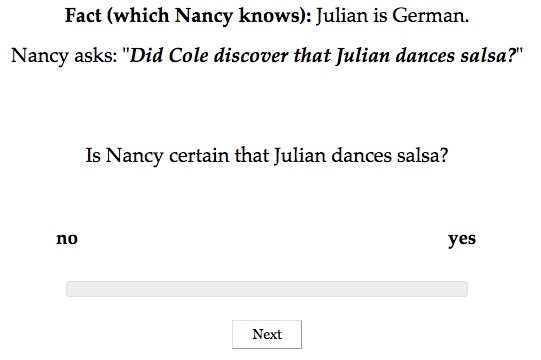
\includegraphics[width=7.9cm]{figures/exp1-projection-trial}} 
\caption{Projection block.}\label{fig-exp1-projection}
 \end{subfigure}%
\begin{subfigure}[t]{0.5\textwidth}
        \centering
\fbox{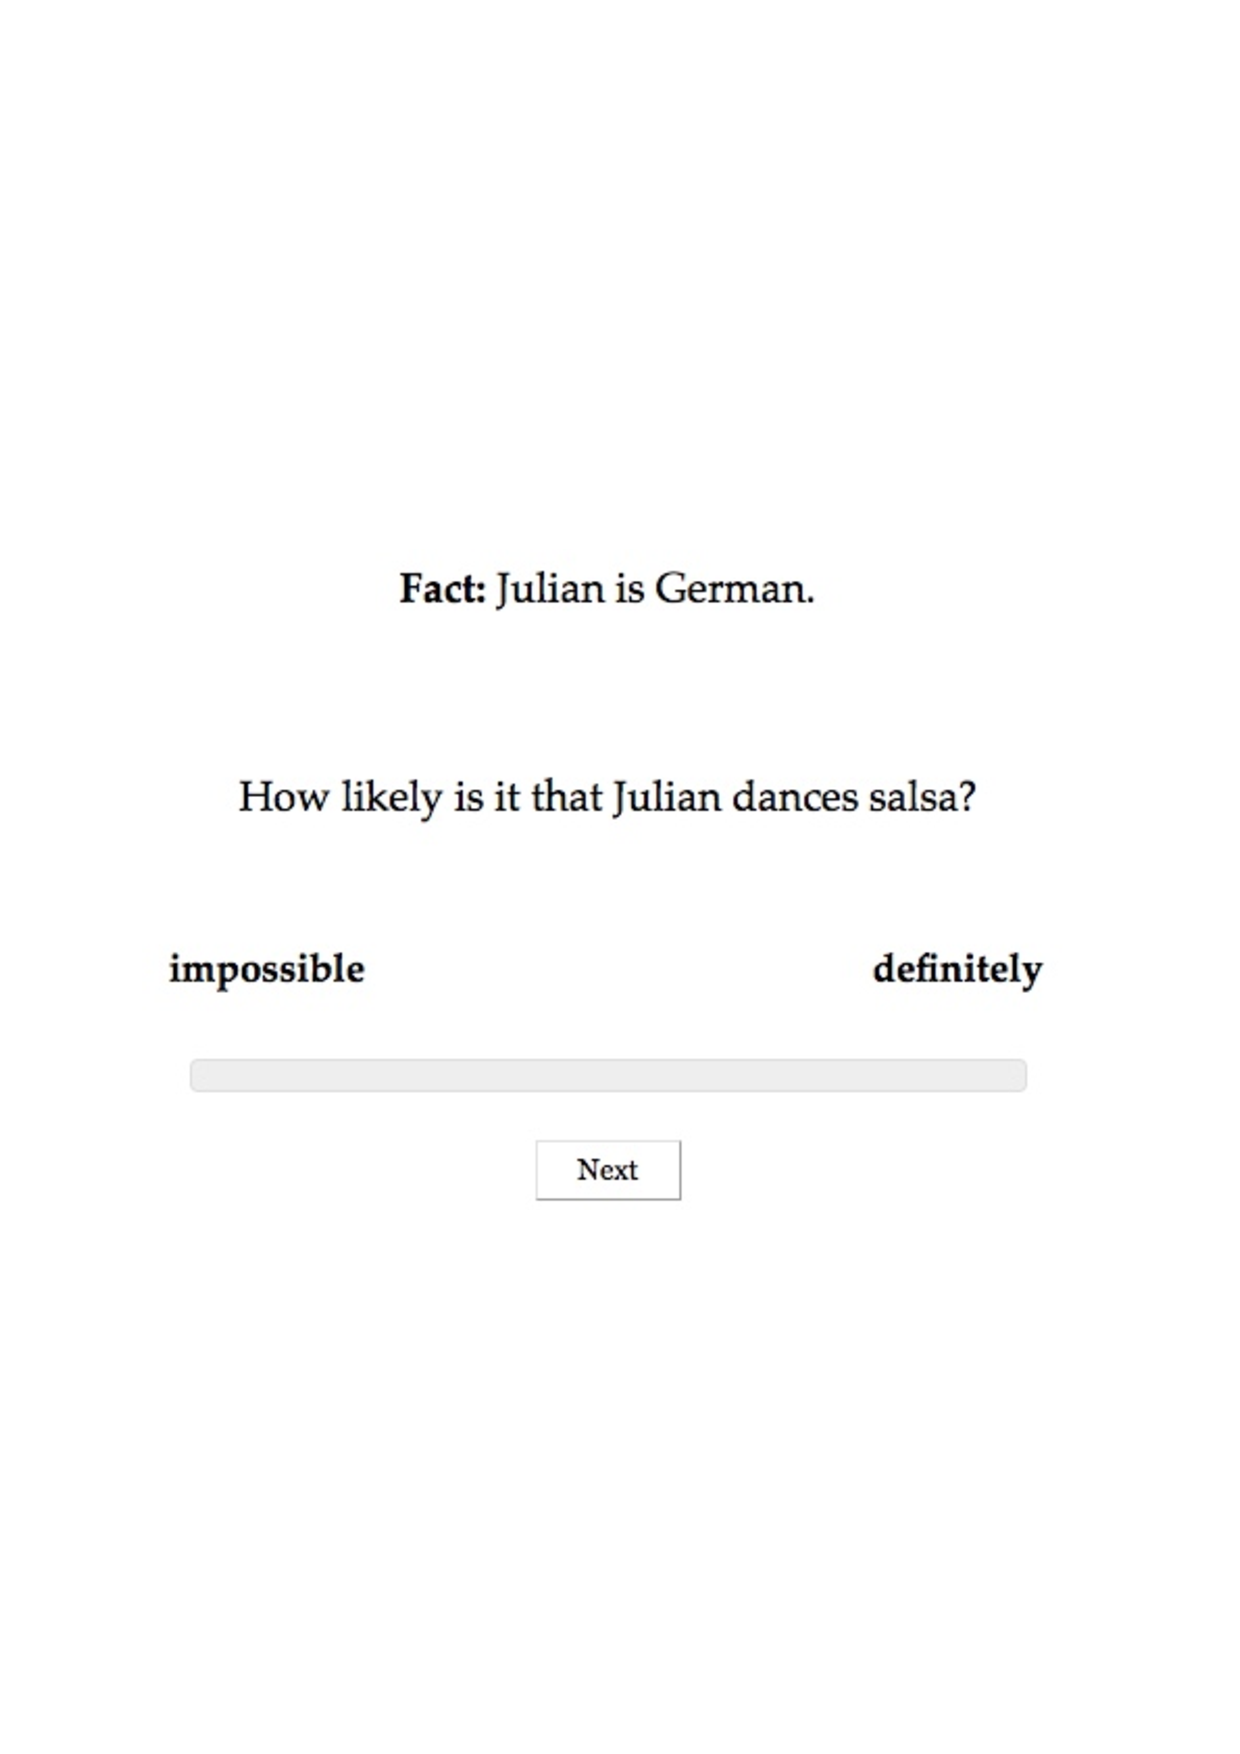
\includegraphics[width=7.55cm]{figures/exp1-prior-trial}}
\caption{Prior block.}\label{f-exp1-prior}
\end{subfigure}
\caption{Sample trials in Exp.~1.}
\end{figure}

After completing the experiment, participants filled out a short, optional survey about their age, their gender, their native language(s) and, if English is their native language, whether they are a speaker of American English (as opposed to, e.g., Australian or Indian English). To encourage them to respond truthfully, participants were told that they would be paid no matter what answers they gave in the survey.

\paragraph{Data exclusion} Prior to analysis, the data from 3 participants who did not self-identify as native speakers of American English were excluded. To assess whether the remaining 297 participants attended to the task, we inspected their responses to the control stimuli. We excluded the data from 11 participants whose response means were more than 2 standard deviations above the group mean. The data from 286 participants (ages 18-82; median: 35.5; 116 female, 186 male, 1 other, 1 undeclared) were analyzed.

\subsection{Results}

We begin by showing that the manipulation of the prior probability of the contents of the 20 clauses was successful, i.e., that the two facts that each of the 20 clauses were presented with indeed influenced the prior probability of the contents of these clauses. To this effect, Figure \ref{f-prior} plots the mean prior probabilities of the contents of the 20 clauses by fact, together with the participants' ratings as light dots. As shown, the mean prior probability of the contents is higher when presented with a higher prior probability fact than when presented with a lower prior probability fact. This finding suggests that our manipulation was successful. 

\begin{figure}[h!]
\centering
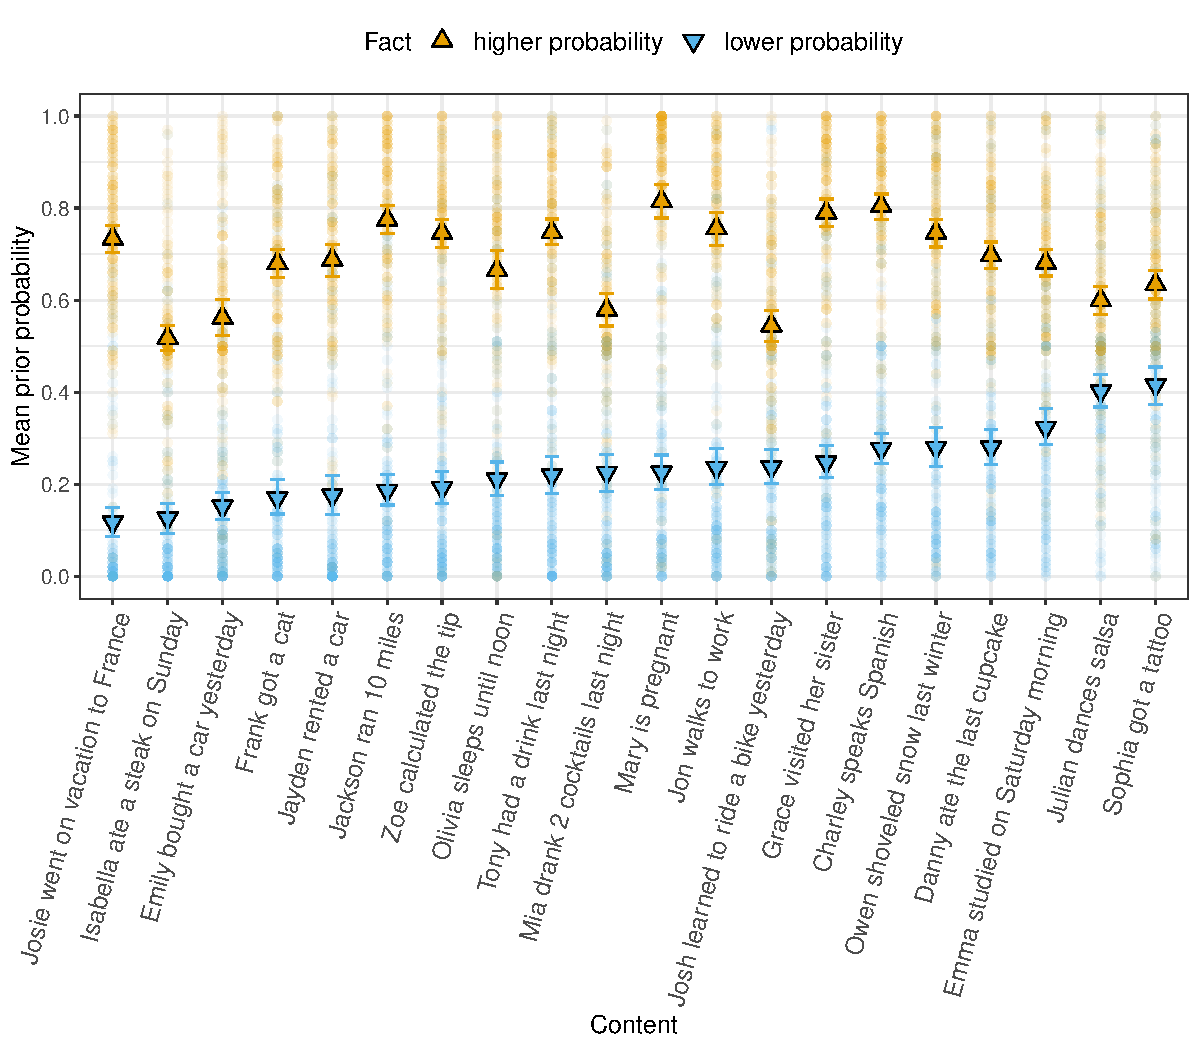
\includegraphics[width=.75\paperwidth]{../../results/exp4/graphs/prior-ratings}

\caption{Mean prior probability by content and fact in Exp.~1. Error bars indicate 95\% bootstrapped confidence intervals. Light dots indicate participants' ratings.} 
\label{f-prior}
\end{figure}

We now address the research question of whether prior probability influences projection. Figure \ref{f-projection-mean} plots the mean certainty ratings for the contents of the clausal complements by clause-embedding predicate and by fact, as well as the mean certainty rating for the main clause content (abbreviated `MC'). Light dots indicate participants' ratings. As shown, the mean certainty ratings were higher for contents  presented with the higher prior probability facts than for contents presented with the lower prior probability fact. This finding, which holds for all 20 clause-embedding predicates, suggests that prior probability influences projection. We also replicate \citepos{tonhauser-degen-factive} finding that there is by-predicate variation in the projection of the content of the complement: for instance, the content of the complement of {\em be annoyed} is more projective than that of {\em discover}, which in turn is more projective than that of {\em announce}. Our experiment provides further evidence for the systematic influence of the predicate on projection: the Spearman rank correlation between the mean certainty ratings for the 20 clause-embedding predicates and the main clause content in our experiment and \citepos{tonhauser-degen-factive} Exp.~1a is .991 (collapsing over facts; see Supplement \ref{a-comparison} for a visualization).

\begin{figure}[h!]
\centering

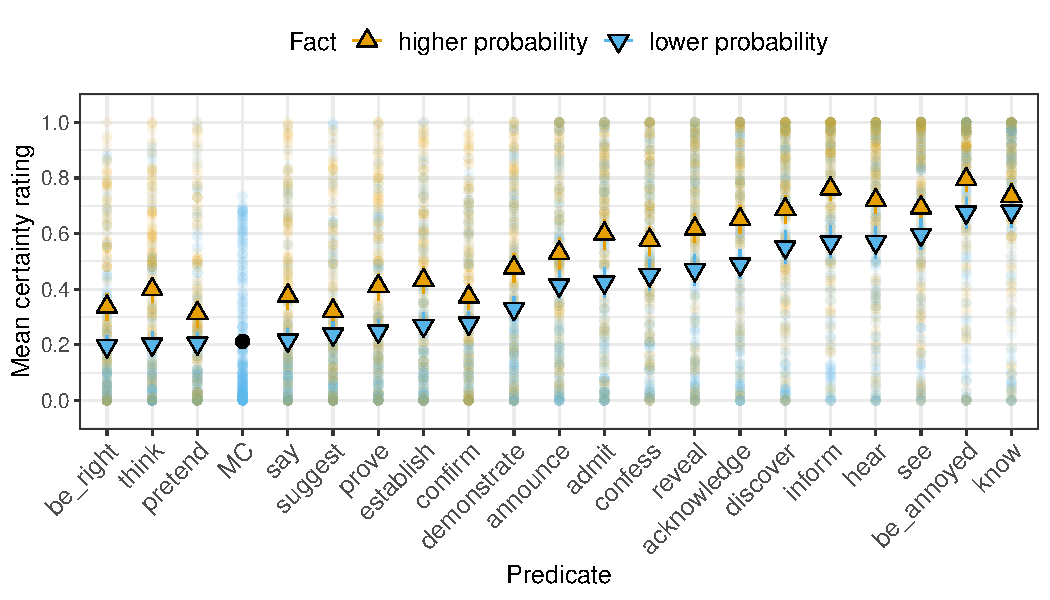
\includegraphics[width=.75\paperwidth]{../../results/exp4/graphs/means-projectivity-by-predicate-and-prior}

\caption{Mean certainty ratings by predicate and prior probability of the content of the complement. Error bars indicate 95\% bootstrapped confidence intervals. Light dots indicate participants' ratings.} 
\label{f-projection-mean}
\end{figure}

Figure \ref{f-projection-mean} plots the certainty ratings according to whether the fact that was presented to the participant was a higher probability fact or a lower probability fact. And although Figure \ref{f-prior} shows that higher and lower probability facts resulted in the expected differences in the mean prior probability ratings for the contents of the 20 clauses, this figure also reveals by-participant variation in prior probability ratings. As a consequence, individual participants' prior probability ratings need not align with the assumed classification. For example, given a particular content (e.g., that Julian dances salsa), it is possible that one participant's prior probability rating was lower than that of another participant, even though the first participant was presented with the higher probability fact (Julian is Cuban) and the second one with the lower probability fact (Julian is German). To investigate whether prior content probability influences projection at the by-participant level, Figure \ref{f-projection} plots the participants' certainty ratings (indicating projection) by their prior probability ratings for the contents of the complements of the 20 clause-embedding predicates. (The color coding here merely presents which type of fact the participant was presented with; no classification is imposed.) The linear smoothers suggest a positive correlation for each predicate between prior probability and certainty ratings such that contents with higher prior probability ratings receive higher certainty ratings. This finding suggests that prior probability predicts projection even at the by-participant level.

\begin{figure}[h!]
\centering

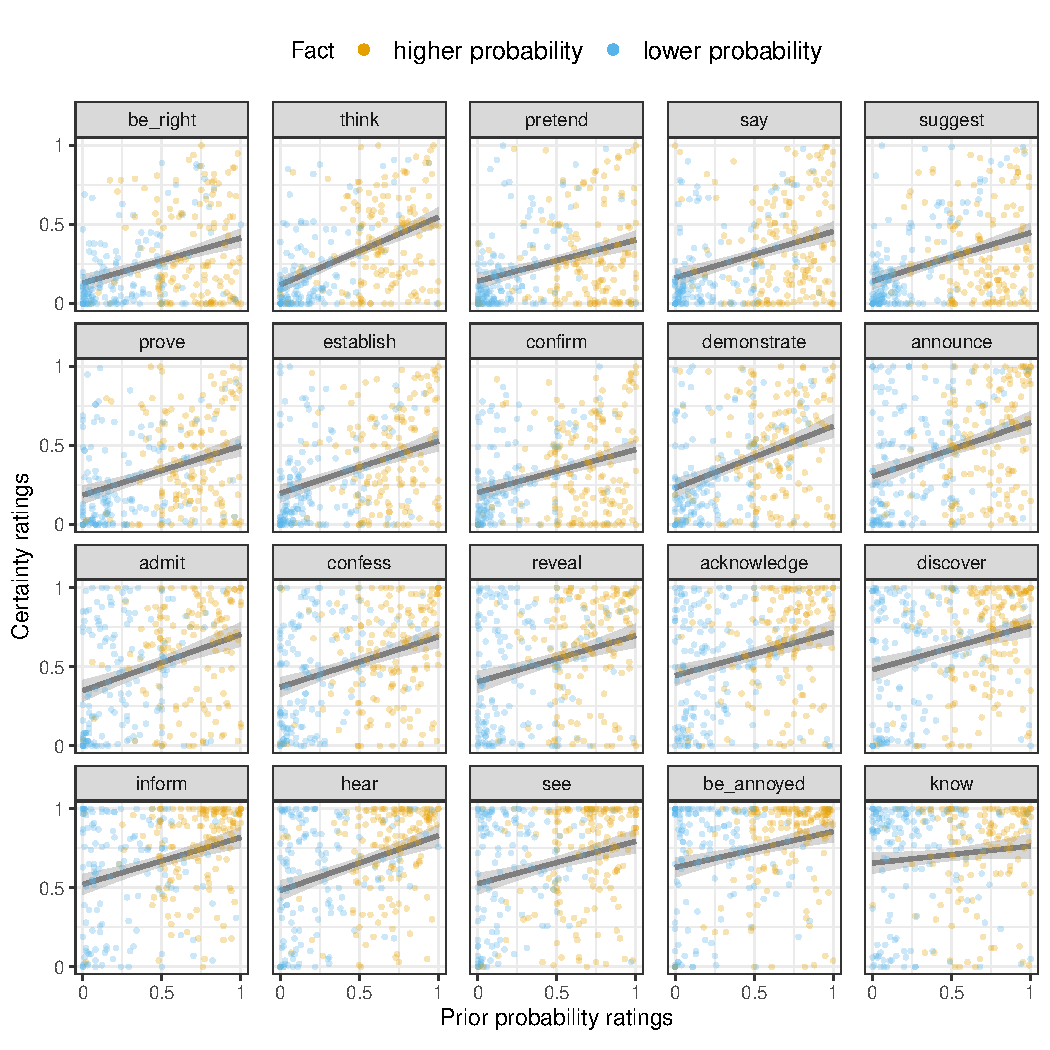
\includegraphics[width=.7\paperwidth]{../../results/exp4/graphs/projection-by-prior}

\caption{Certainty ratings by prior probability ratings by predicate in Exp.~1. Linear smoothers with 95\% confidence intervals are overlaid.}
\label{f-projection}
\end{figure}

\newpage

The qualitative observations about the relations between prior probability, clause-embedding predicate and projection were borne out statistically. We fitted a Bayesian mixed effects Beta regression model  with weakly informative priors using the \verb|brms| \citep{buerkner2017}  package in R \citep{R} on the target data (5,720 data points). The model predicted the certainty ratings from a fixed effect of prior probability and included the maximal random effects structure justified by the design, namely random by-participant and by-item intercepts (where an item is a combination of a predicate and a complement clause). A Beta regression model estimates the mean of the outcome distribution (like a linear regression model).\footnote{Beta regression models also estimate a second parameter, namely the precision, which is a measure of dispersion: the greater the precision, the more concentrated the ratings are around the mean. In this paper, we rely on the estimated mean to identify whether prior probability predicts projection. Both the estimated mean and precision are reported in the full model output table in Supplement \ref{modeldetails}.} We thus obtain a 95\% credible interval for \jt{the mean effect of prior probability on certainty?}. Supplement \ref{modeldetails} motivates the use of Beta regression over linear regression, provides a brief primer on how to interpret Bayesian mixed effects Beta regression models, and reports the full model output.

\jt{According to the Beta regression model, the estimated mean for each predicate was higher than that of the main clause controls, i.e., the 95\% credible intervals for the estimated adjustment to the main clause control mean did not contain 0 for any predicate. This suggests that the content of the complement of each of the 20 predicates is projective compared to non-projective main clause content.\footnote{\jt{A Bayesian mixed effects linear regression with the same fixed and random effects structure yielded qualitatively identical results, except that the contrast between \emph{pretend} and the main clause controls was only marginally significant. See the Github repository mentioned in footnote \ref{f-github} for the model code.}} Thus, to distinguish factive predicates from optionally factive and non-factive ones in this set of 20 predicates, one would need to arbitrarily distinguish one group of projective CCs from another group of projective CCs.} 

\newpage


\subsection{Discussion}

The findings of Exp.~1 provide empirical support for the hypothesis, put forth in \citealt{stevens-etal2017} and \citealt{tbd-variability}, that the prior probability of content influences its projection. Specifically, we observed that a participant's certainty ratings for the content of the clausal complement of a predicate like {\em think, announce} and {\em know} are influenced by the prior probability rating for such content.

{\bf Lorson:} There are several differences between Exp.~1 and \citepos{lorson2018} investigation that may have contributed to why \citealt{lorson2018} did not observe an influence of prior probability on projection. 

\begin{enumerate}

\item Difference: \citealt{lorson2018} did not collect by-participant prior ratings in addition to certainty ratings but relied on the ratings obtained in previous work. It is possible that her participants did not differ in prior probability. \jt{Should this be part of the motivation/section 1?}


\item Difference: the prior probability of content was manipulated through gender stereotypes in \citealt{lorson2018} but assumptions about what individuals with a variety of dispositions, professions, ages or nationalities are more or less likely to do. As shown in Figure \ref{f-influence-by-content}, the effect of prior probability on projection is observed for all contents, i.e., regardless of how prior probability was manipulated.

\begin{figure}[h!]
\centering

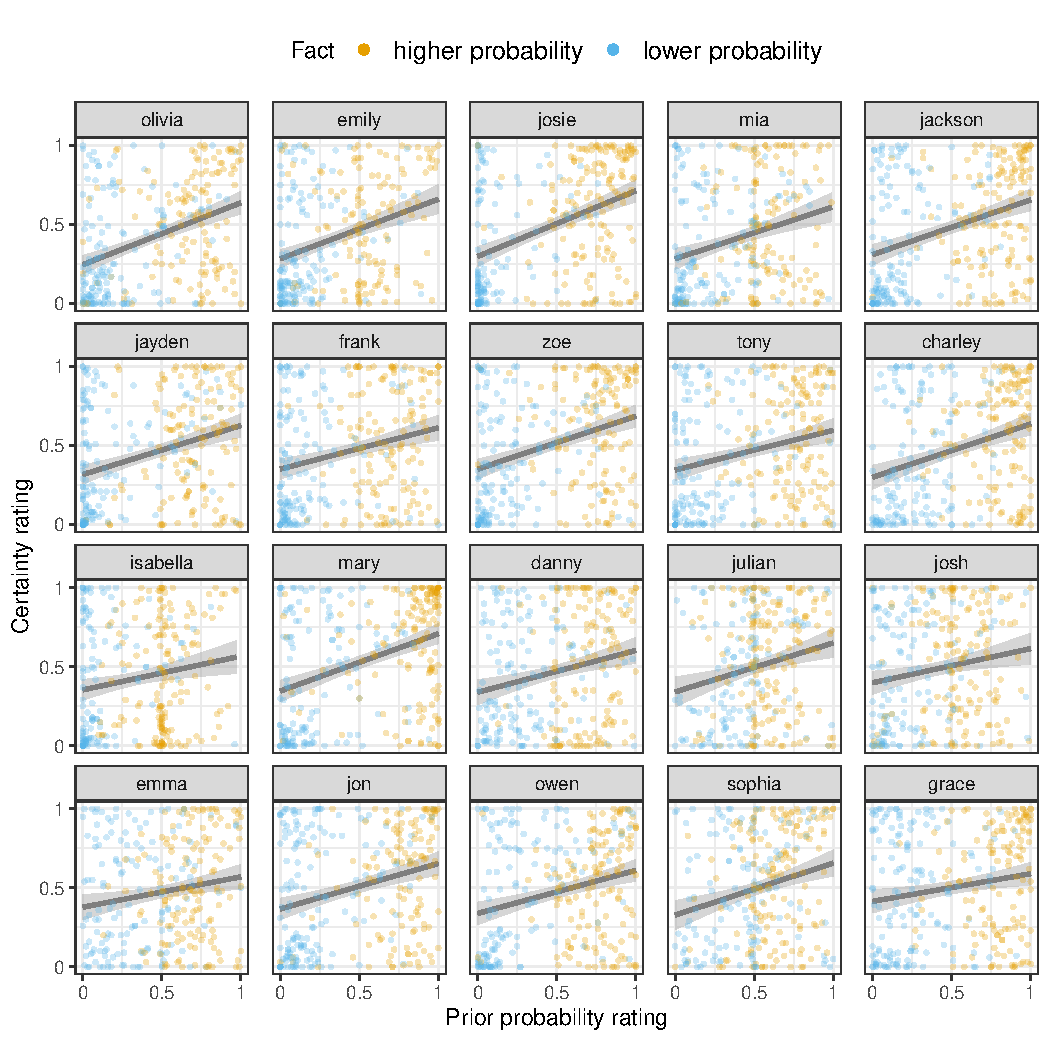
\includegraphics[width=.7\paperwidth]{../../results/exp4/graphs/projection-by-prior-by-content}

\caption{Certainty ratings by prior probability ratings by content in Exp.~1. Linear smoothers with 95\% confidence intervals are overlaid.}
\label{f-influence-by-content}
\end{figure}

\item Difference: we investigated the projection of the content of the clausal complement of clause-embedding predicates whereas \citealt{lorson2018} investigated the pre-state content of {\em stop}. \jt{How much to investigate this possibility?}

\end{enumerate}

{\bf Mahler:} found an effect based on a manipulation of prior probability based on content that was more or less likely depending on the political party affilliation. 

\begin{enumerate}

\item We replicate her finding, showing that it generalizes to prior probability manipulated based on a broader variety of properties of individuals. \jt{May also be a good reason to include Fig 5}

\item Mahler used the content of the complement of clause-embedding predicates, like us. She had 7 predicates; we had 20. She found that the CCs of factive predicates more projective than CCs of non-factive predicates, and finds the effect for both groups (no by-predicate discussion). We go beyond her by showing that this holds for 20 predicates.

\item ``CCs were more projective when the predicate was factive compared to when it was non-factive, regardless of the speaker?s political affiliation. This finding is compatible with the assumption that factive predicates lexically-encode their complements as presuppositions, whereas non-factive predicates do not.'' (p.788) \jt{We want to engage with this here: factives paper challenges factive/non-factive distinction so the fact that we find effect of prior on all predicates cannot be used to support such a differential analysis}

\end{enumerate}

Possible that participants' responses on either block primed their responses on the other block, so we also conduced experiment where prior probability ratings were collected from a different population.

\section{Experiment 2: Prior probability}

This experiment collected prior probability ratings for the 20 contents.

\subsection{Methods}

\paragraph{Participants} 95 participants with U.S.\ IP addresses and at least 99\% of previous HITs approved were recruited on Amazon's Mechanical Turk platform (ages: 21-75, median: 33; 45 female, 50 male). They were paid 55 cents for participating. 

\paragraph{Materials} The 40 target stimuli were identical to the target stimuli of the prior block of Exp.~1. For each participant, a random combination of 20 clause/fact combinations was generated, for 20 target stimuli. Each participant also saw the two control stimuli in (\ref{control}), which were included to assess whether participants were attending to the task: we expected participants to rate the prior probability of the content in (\ref{control}a) as high and that of the content in (\ref{control}b) as low. Trial order of the 22 stimuli was random.

\begin{exe}
\ex\label{control2}
\begin{xlist}
\ex {\bf Fact:} Barry lives in Germany. \\ How likely is it that Barry lives in Europe?
\ex {\bf Fact:} Tammy is a rabbit. \\ How likely is it that Tammy speaks Italian and Greek?
\end{xlist}
\end{exe}

\paragraph{Procedure} The procedure was identical to the procedure of the prior block of Exp.~1. After completing the experiment, participants filled out the same optional survey as in Exp.~1.

\paragraph{Data exclusion} Prior to analysis, the data from 8 participants who did not self-identify as native speakers of American English were excluded. To assess whether the remaining 87 participants attended to the task, we inspected their responses to the 2 control stimuli. The response means of 12 participants were more than 2 standard deviations below the group mean of the control in (\ref{control}a) or more than 2 standard deviations above the group mean of the control in (\ref{control}b). We excluded the data from these participants, leaving data from 75 participants (ages 21-75; median: 35; 34 female, 41 male).

\subsection{Results and discussion}

\jt{Is the effect of prior on projection an artifact of the ratings collected in Exp1? predict projection mean from prior mean in both Exp1 and with Exp2 prior ratings, for comparing the two experiments; use cohen?s d?}

Figure \ref{f-prior-comparison} plots the mean prior probability ratings in Exp.~2 against the mean prior probability ratings in Exp.~2.  \jt{what do we see?}

Spearman rank correlation: .98

\begin{figure}[H]
\centering

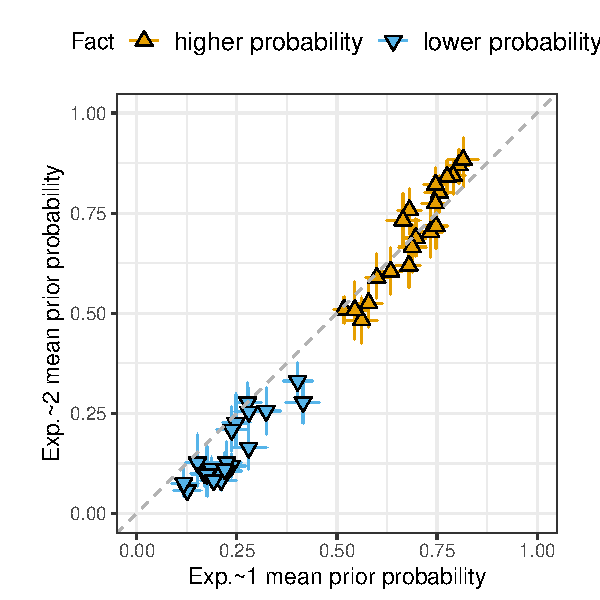
\includegraphics[width=.5\paperwidth]{../../results/1-prior/graphs/prior-probability-comparison-exp1-exp2}

\caption{Mean prior probability ratings in Exp.~2 against those of Exp.~1. Error bars indicate 95\% bootstrapped confidence intervals.}
\label{f-prior-comparison}
\end{figure}

\jt{Report model that predicts projection of Exp.~1 projection data from the new prior probability means.}


\section{Discussion}\label{s4}


as well as for the main clause stimuli (abbreviated `MC'), in increasing order from left to right. The mean certainty ratings are largely consistent with impressionistic judgments reported in the literature. First, the ratings for main clause content are lowest overall, as expected for non-projective content. Second, the ratings for factive predicates are among the highest overall, suggesting comparatively high projectivity of the CC. Third, the mean certainty ratings of many optionally factive predicates are lower than those of many factive predicates and higher than those of main clauses as well as of non-veridical non-factives. However, Figure \ref{f-projectivity} also shows that the CCs of the 5 predicates assumed to be factive are not categorically more projective than the CCs of the optionally factive predicates, contrary to what is expected under the first definition of factive predicates. Specifically, the CCs of the optionally factive predicates {\em acknowledge, hear} and {\em inform} are at least as projective as the CCs of {\em reveal} or {\em discover}. This finding suggests that projectivity alone does not categorically distinguish factive predicates from optionally factive and non-factive ones.


These results support \citetpos{tbd-variability} hypothesis that prior content probability influences projectivity. The finding that the CC of many non-factive predicates is at least weakly projective, even with low prior probability CCs, confirms intuitions reported in, e.g., \citealt{schlenker10}, \citealt{anand-hacquard2014} and \citealt{spector-egre2015}. These findings motivate the development of projection analyses that derive the influence of prior content probability and make predictions for the CCs of a broad range of both factive and non-factive predicates.

Current projection analyses, while limited to the CCs of factive predicates (e.g., \citealt{heim83,vds92,abrusan2011,brst-salt10,brst-ar}), are compatible with the finding that prior content probability influences projectivity. \citealt{heim83}, for instance, assumes default global accommodation when a presupposition is not entailed by the common ground (CG) when the trigger is uttered. This default is overridden when the presupposition is inconsistent with the CG. If we can assume that Julian dancing salsa is more likely to be consistent with the CG when Julian is Cuban than when he is German, \citealt{heim83} predicts that the presupposition that Julian dances salsa is more projective when it has a higher prior probability. 

As shown in Fig.~\ref{f-proj}, the CCs of several non-factives, including {\em inform, hear, acknowledge} and {\em admit}, are at least as projective as that of factive {\em reveal}. This finding challenges the long-standing assumption that the CCs of factives are more projective than those of non-factives. We suggest that this motivates constraint-based analyses that derive the projectivity of utterance content from the integration of multiple cues, including prior CC probability, the meanings of clause-embedding predicates, at-issueness (\citealt{tbd-variability}), and information structure (\citealt{tonhauser-salt26}).

{\bf discussion:} measure prior and projection at participant-level (as we do in next work)

\section{Conclusions}\label{s5}



\bibliographystyle{/Users/tonhauser.1/Library/Latex/cslipubs-natbib}
\bibliography{/Users/tonhauser.1/Documents/bibliography}

\newpage

\appendix

\setcounter{table}{0}
\renewcommand{\thetable}{A\arabic{table}}

\setcounter{figure}{0}
\renewcommand{\thefigure}{A\arabic{figure}}

\section*{Supplemental material for {\em Higher-probability content is more projective than lower-probability content}}

\section{Experiment 1 target and control stimuli}\label{a-stim}

The target stimuli of the projection block of Exp.~1 consisted of 800 combinations of a predicate, a complement clause and a fact relative to which the content of the complement clause had a higher or lower probability. The following list gives the 20 clauses that served as complement clauses together with the two facts that the clause was paired with: first the lower probability fact, then the higher probability one. The target stimuli of the prior block of Exp.~1 consisted of the 40 combinations of a clause and a fact.

\begin{enumerate}[leftmargin=3ex,itemsep=-2pt]
\item Mary is pregnant (Mary is a middle school student / Mary is taking a prenatal yoga class)
\item Josie went on vacation to France (Josie doesn't have a passport / Josie loves France)
\item Emma studied on Saturday morning (Emma is in first grade / Emma is in law school)
\item Olivia sleeps until noon (Olivia has two small children / Olivia works the third shift)
\item Sophia got a tattoo (Sophia is a high end fashion model / Sophia is a hipster)
\item Mia drank 2 cocktails last night (Mia is a nun / Mia is a college student)
\item Isabella ate a steak on Sunday (Isabella is a vegetarian / Isabella is from Argentina)
\item Emily bought a car yesterday (Emily never has any money / Emily has been saving for a year)
\item Grace visited her sister (Grace hates her sister / Grace loves her sister)
\item Zoe calculated the tip (Zoe is 5 years old / Zoe is a math major)
\item Danny ate the last cupcake (Danny is a diabetic / Danny loves cake)
\item Frank got a cat (Frank is allergic to cats / Frank has always wanted a pet)
\item Jackson ran 10 miles (Jackson is obese / Jackson is training for a marathon)
\item Jayden rented a car (Jayden doesn't have a driver's license / Jayden's car is in the shop)
\item Tony had a drink last night (Tony has been sober for 20 years / Tony really likes to party with his friends)
\item Josh learned to ride a bike yesterday (Josh is a 75-year old man / Josh is a 5-year old boy)
\item Owen shoveled snow last winter (Owen lives in New Orleans / Owen lives in Chicago)
\item Julian dances salsa (Julian is German / Julian is Cuban)
\item Jon walks to work (Jon lives 10 miles away from work / Jon lives 2 blocks away from work)
\item Charley speaks Spanish (Charley lives in Korea / Charley lives in Mexico)
\end{enumerate}

In the target stimuli of the projection block of Exp.~1, eventive predicates, like {\em discover} and {\em hear}, were realized in the past tense and stative predicates, like {\em know} and {\em be annoyed}, were realized in the present tense. The direct object of {\em inform} was realized by the proper name {\em Sam}. The subject of the clause-embedding predicate and the speaker of the target stimuli were realized by a proper name. 

\bigskip
\noindent
The following list gives the six control stimuli of the projection block of Exp.~1: 

\begin{enumerate}[leftmargin=3ex,itemsep=-2pt]
\ex {\bf Fact:}  Zack is a member of the golf club. Is Zack coming to the meeting tomorrow?

\ex  {\bf Fact:} Mary visited her aunt on Sunday. Is Mary's aunt sick?

\ex  {\bf Fact:} Todd goes to the gym 3 times a week. Did Todd play football in high school?

\ex  {\bf Fact:} Vanessa won a prize at school. Is Vanessa good at math?

\ex  {\bf Fact:} Trish sent Madison a card. Did Madison have a baby?

\ex  {\bf Fact:} Hendrick just bought a car. Was Hendrick's car expensive?
\end{enumerate}

\section{Model details for Experiments 1, 2 and 3}\label{modeldetails}

This supplement provides details on the data analysis conducted for Exps.~1, 2, and 3. We first motivate the use of Beta regression rather than linear regression in Exps.~1a, 2a, and 3a (section \ref{a-motivation}) and then provide a brief primer on how to interpret Bayesian mixed effects Beta regression models (section \ref{a-primer}). We then report the model outputs for Exps.~1, 2, and 3 (section \ref{a-mo}).

\subsection{Motivation for using Bayesian mixed effects Beta regression}\label{a-motivation}

There are three separate pieces to motivate: the use of \emph{mixed effects}, the use of a \emph{Bayesian} rather than \emph{frequentist} models, and the use of \emph{Beta regression} rather than \emph{linear regression}. 

\textbf{Using mixed effects} refers to the practice of modeling the outcome variable, here slider ratings or proportions of `yes' ratings, as a function of not just fixed effects of interest (i.e., predicate) but also as the result of possible random variability that is not of theoretical interest (e.g., random by-participant or by-item variability). This is standard practice in psycholinguistic studies and allows the researcher to trust that any observed effects of theoretical interest are true average effects rather than the result of idiosyncratic behavior (e.g., of participants or items). This is also the motivation for using mixed effects in Exps.~1b, 2b, and 3b.

\textbf{Using Bayesian models} rather than frequentist models is increasingly becoming the norm in psycholinguistic studies as computational power has increased and running Bayesian models has become more accessible with the introduction of R packages such as \verb|brms| \citep{buerkner2017}. The presence of an effect in frequentist models is evaluated by checking whether the {\em p-}value is smaller than $.05$, where the {\em p-}value is defined as the probability of obtaining data that is as skewed or more skewed than the observed data if the null-hypothesis was true, i.e., if the hypothesized effect was absent. Parameter estimates in frequentist models are obtained via maximum-likelihood techniques, i.e., by estimating the parameter values that maximize the probability of observing the data. Bayesian models, by contrast, return a full posterior distribution over parameter values that take into account not just the probability of the data under the parameter values, but also the prior probability of parameter values. In order to evaluate the evidence for an effect of a predictor of interest, one can report 95\% credible intervals and the posterior probability $P(\beta < 0)$ or $P(\beta > 0)$ that the predictor coefficient $\beta$ is either lower or greater than zero, depending on the direction of the expected effect. A 95\% credible interval (CI) demarcates the range of values that comprise 95\% of probability mass of the posterior beliefs such that no value inside the CI has a lower probability than any point outside it \citep{Jaynes1976, Morey2016}. There is substantial evidence for an effect if zero is (by a reasonably clear margin) not included in the 95\% CI and $P(\beta > 0)$ or $P(\beta < 0)$ is close to zero or one. Posterior probabilities indicate the probability that the parameter has a certain value, given the data and model -- these probabilities are thus \emph{not} frequentist {\em p-}values. In order to present statistics as close to widely used frequentist practices, and following \citealt{Nicenboim2016}, we defined an inferential criterion that seems familiar (95\%), but the strength of evidence should not be taken as having clear cut-off points (such as in a null-hypothesis significance testing framework).

\textbf{Using Beta regression} rather than linear regression was motivated by the violation of two of the  assumptions of linear regression: first, that residuals be normally distributed (where ``residuals'' refers to the residual error for each data point after fitting the model), and second, that the error term exhibit homoscedasticity (that it be roughly the same across different conditions). Slider ratings data has the property of being bounded by its endpoints (which we code as 0 and 1, respectively). This often leads to ``bunching'' behavior at the endpoints (see Figure \ref{fig:bunch} for the distribution of raw ratings in Exps.~1a, 2a, and 3a). 


\begin{figure}[h!]
\begin{subfigure}{.33\textwidth}
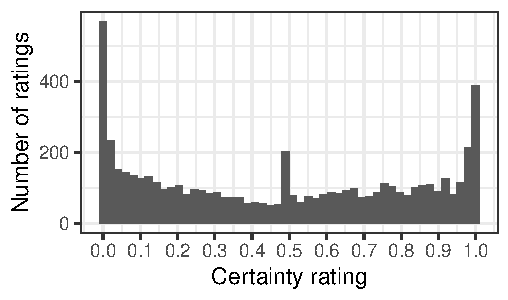
\includegraphics[width=\textwidth]{../../results/exp4/graphs/bunching-projection}
\caption{Exp.~1 certainty ratings.}
\label{fig:exp1araw}
\end{subfigure}
\begin{subfigure}{.33\textwidth}
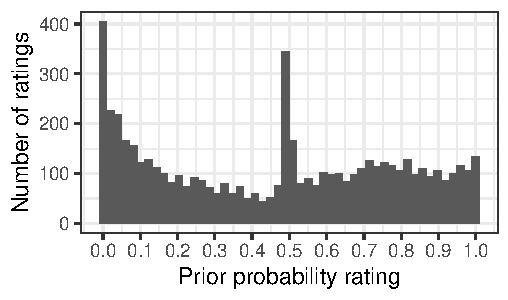
\includegraphics[width=\textwidth]{../../results/exp4/graphs/bunching-prior}
\caption{Exp.~1 prior ratings.}
\label{fig:exp2araw}
\end{subfigure}
\begin{subfigure}{.33\textwidth}
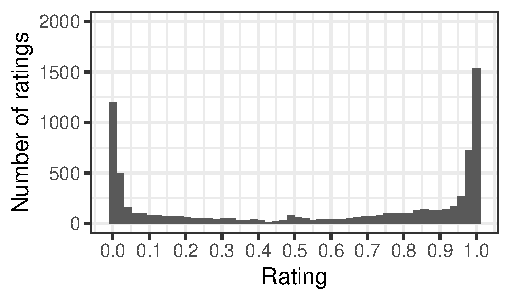
\includegraphics[width=\textwidth]{../../results/2-veridicality2/graphs/bunching}
\caption{Exp.~2 prior ratings.}
\label{fig:exp3araw}
\end{subfigure}
\caption{Histograms of raw slider ratings in Exps.~1 and 2.}
\label{fig:bunch}
\end{figure}

This ``bunching'' behavior, in turn, can lead to the violation of both of the above assumptions of linear regression. 
Intuitively, these assumptions are violated because conditions that elicit ratings closer to endpoints necessarily have a compressed variance; consequently, a condition's mean and its variance are not independent. Beta regression is useful here because it allows for modeling an arbitrarily distributed outcome variable in the $[$0,1$]$ interval. The Beta distribution is characterized by two parameters, one capturing the mean $\mu$ of the distribution and one capturing its precision $\phi$, a measure of dispersion. The greater the precision, the more concentrated the values are around the mean, i.e., the lower the variance of the distribution.  We follow \citet{smithson2006} in modeling $\mu$ and $\phi$ separately for each predictor. That is, we allow each predictor to affect both the mean and the precision of the outcome variable's distribution. 

\subsection{Coding choices and interpreting model output}\label{a-primer}

The outcome variable in Exps.~1a, 2a and 3a (slider ratings) contained the values 0 and 1, which Beta regression is undefined for. We therefore applied a common transformation to ratings before the main analysis that rescales values $y$ to fall in the open unit interval (0,1)  \citep{smithson2006}. First, we apply $y' = (y-a)/(b-a)$, where $b$ is the highest possible slider rating and $a$ is the smallest possible slider rating. The range is then compressed to not include 0 and 1 by applying $y'' = [y'(N-1) + 1/2]/N$, where $N$ is the total number of observations.

The mean parameter $\mu$ is modeled via a logit link function (default for Beta regression in \verb|brms|), though other links that squeeze $\mu$ into the $[$0,1$]$ interval are possible. The dispersion parameter $\phi$ is modeled via a log link, which ensures that values of $\phi$ are strictly positive, which is necessary because a variance cannot be negative. 

We allowed both $\mu$ and $\phi$ to vary as a function of predicate, with reference level set to main clause control in Exp.~1a, entailing control in Exp.~2a and contradictory control in Exp.~3a. We also allowed random intercept adjustments to each parameter by participant and by item, where item was defined as a unique combination of a predicate and a complement clause. Four chains converged after 2000 iterations each (warmup = 1000, \(\hat{R}=1\) for all estimated parameters) with a target acceptance rate of .95 and a maximum treedepth of 15.

\subsection{Model outputs for Experiments 1, 2 and 3}\label{a-mo}

The three tables in this section show the model outputs for Exps.~1, 2 and 3, respectively: Table \ref{tab:exp1modelresults} for Exps.~1a and 1b, Table \ref{tab:exp2modelresults} for Exps.~2a and 2b, and Table \ref{tab:exp3modelresults} for Exps.~3a and 3b. Each table shows maximum a posteriori (MAP) model estimates for projection ratings from the Beta regression model (left and middle column, mean $\mu$ and precision $\phi$) and the logistic regression model (right column, $\beta$)  with 95\% credible intervals.

\section{Projection comparison}\label{a-comparison}

Projection: Comparison of findings of Exp.~1 and \citepos{tonhauser-degen-factive} Exp.~1a

\begin{figure}[H]
\centering

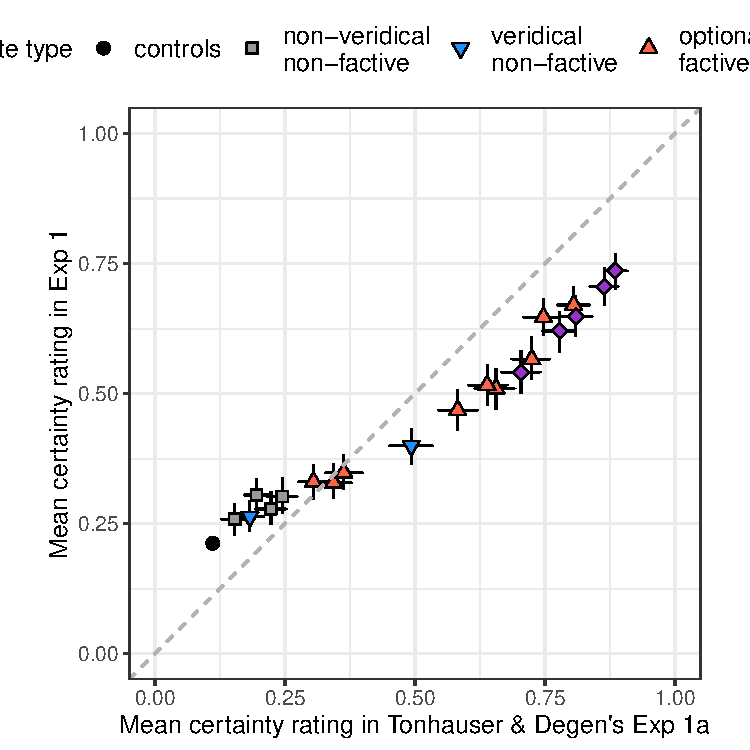
\includegraphics[width=.4\paperwidth]{../../results/exp4/graphs/projection-comparison}

\caption{Mean by-predicate certainty ratings in Exp.~1 and \citepos{tonhauser-degen-factive} Exp.~1a. Error bars indicate 95\% bootstrapped confidence intervals.} 
\label{f-projection-comparison}
\end{figure}

\section{Projection experiment}\label{a-proj}

\subsection{Methods}

\paragraph{Participants} 300 participants with U.S.\ IP addresses and at least 99\% of previous HITs approved were recruited on Amazon's Mechanical Turk platform (ages: 21-72, median: 36; 145 female, 154 male, 1 undeclared). They were paid 85 cents for participating. 

\paragraph{Materials and procedure} The materials and procedure of this experiment were identical to those of the projection block of Exp.~1. 

\paragraph{Data exclusion}
Prior to analysis, the data from 23 participants who did not self-identify as native speakers of American English were excluded. To assess whether the remaining 277 participants attended to the task, we inspected their responses to the 6 control stimuli. There were 11 participants whose response means were more than 2 standard deviations above the group mean. We excluded the data from these participants, too, leaving data from 266 participants (ages 21-72; median: 36; 129 female, 136 male, 1 undeclared).

\subsection{Results}

Figure \ref{f-projection2} shows the mean certainty ratings for the target stimuli by predicate and by the prior probability of the content of the complement; the mean certainty rating for the non-projective main clause controls are also included. As shown, mean certainty ratings were higher when the content had a higher prior probability than when it had a lower prior probability, as hypothesized by \citet{tbd-variability}. This finding suggests that prior content probability influences projection. Furthermore, the effect of prior content probability on projectivity was present across all 20 clause-embedding predicates.

\begin{figure}[H]
\centering

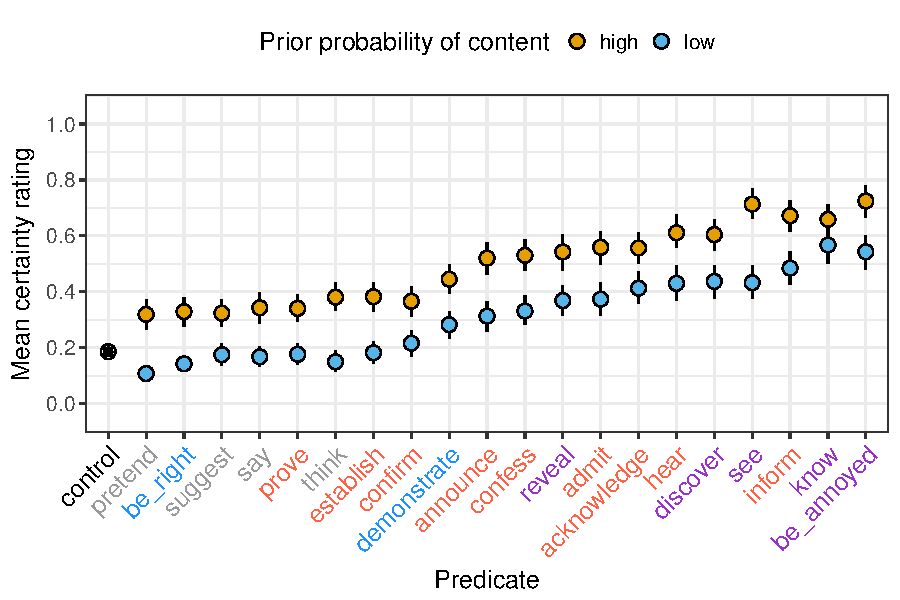
\includegraphics[width=.75\paperwidth]{../../results/3-projectivity/graphs/means-projectivity-by-predicate-and-facttype}

\caption{Mean certainty ratings by predicate and prior probability of the content of the complement. Error bars indicate 95\% bootstrapped confidence intervals.} 
\label{f-projection2}
\end{figure}

\jt{report analyses here: prior from Exp1/projection from this experiment}

\end{document}

